\subsection{Badania przesiewowe dla średniej ilości neuronów}
Eksperyment ten miał na celu sprawdzenie jak zachowuje się sieć przy średniej ilości neuronów w dwóch warstwach. Wszystkie parametry pozostały bez zmian, zmieniana była jedynie ilość neuronów w zakresie od 10 do 100 z krokiem 10.
\begin{figure}[!h]
\centering
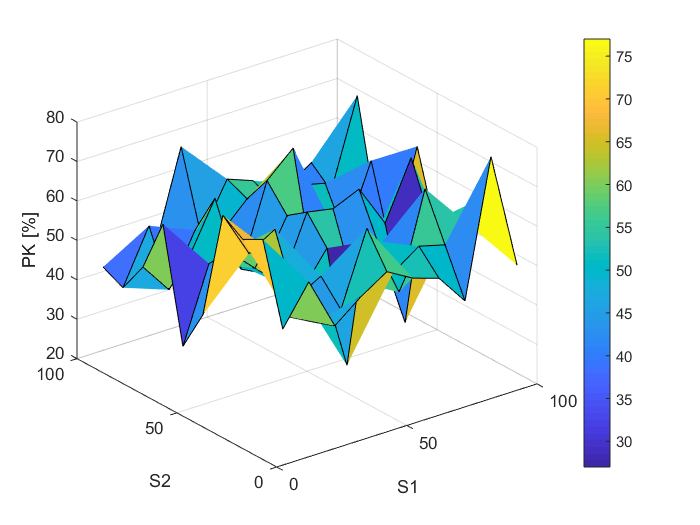
\includegraphics[width = 0.65\textwidth]{Grafika/pk_srednie.png}
\caption{Wpływ liczby neuronów w warstwie pierwszej i drugiej na poprawność klasyfikacji}
\label{fig:PKeksperyment3}
\end{figure}
\begin{figure}[!h]
\centering
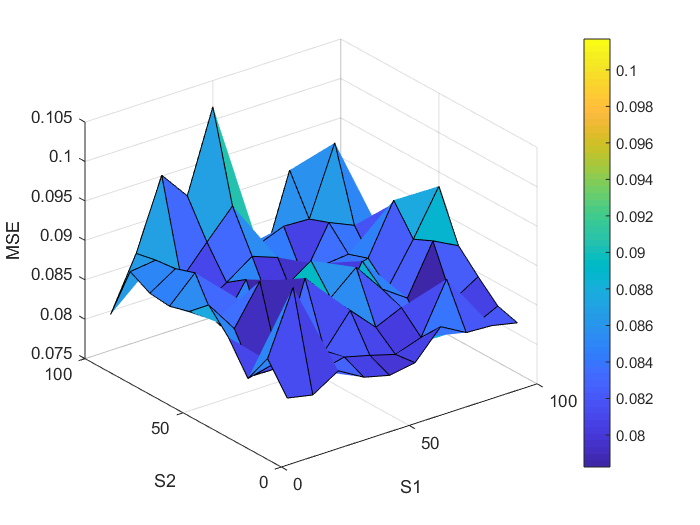
\includegraphics[width = 0.65\textwidth]{Grafika/mse_srednie.png}
\caption{Wpływ liczby neuronów w warstwie pierwszej i drugiej na błąd średnio-kwadratowy}
\label{fig:MSEeksperyment3}
\end{figure}

Największą poprawność klasyfikacji ($57.38\%$) uzyskano dla 250 neuronów w warstwie pierwszej i 100 w warstwie drugiej.\\
Najmniejszy błąd średnio-kwadratowy ($0.0834284$) osiągnięty został dla 300 neuronów w warstwie pierwszej i 100 neuronów w warstwie drugiej. Dla tej konfiguracji $PK$ wyniosło $54.63\%$.\\